%-%-%-%-%-%-%-%-%-%-%-%-%-%-%-%-%-%-%-%-%-%-%-%-%-%-%-%-%-%-%-%-%-%-%-%-%-%-%
%%% MAIN DOCUMENT %%%

%-%-%-%-%-%-%-%-%-%-%-%-%-%-%-%-%-%-%-%-%-%-%-%-%-%-%-%-%-%-%-%-%-%-%-%-%-%-%

\documentclass[12pt]{article}
\usepackage{xcolor}
\usepackage{minted}

% \usepackage[T1]{fontenc}

\usepackage{draculatheme}
\newcommand{\documentTheme}{draculafg}
\newcommand{\documentLogo}{../../images/small logo_white.png}
\newcommand{\documentBigLogo}{../../images/logo_white_text.png}
\usemintedstyle{dracula}

\usemintedstyle{dracula}

\setminted{
    linenos=true,
    numbersep=5pt,
    frame=lines,
    framesep=2mm,
    breaklines=true
}

% \newcommand{\documentBigLogo}{../../images/Hendrix Logo.png}
% \newcommand{\documentLogo}{../../images/small logo.png}
% \newcommand{\documentTheme}{black}

%%% AESTHETICS %%%
%-%-%-%-%-%-%-%-%-%-%-%-%-%-%-%-%-%-%-%-%-%-%-%-%-%-%-%-%-%-%-%-%-%-%-%-%-%-%


%%% Dimensions and Spacing %%%
\usepackage[margin=1in]{geometry}
\usepackage{setspace}
\usepackage{mathtools}
\usepackage{esint}
\usepackage{adjustbox}
\linespread{1}
\usepackage{listings}
\usepackage{tikz}
\usetikzlibrary{shapes,backgrounds,calc,patterns,positioning}
\usepgflibrary{shadings}
\usepackage{pgfkeys}
\usepackage{pdftexcmds}
\usepackage{shellesc}
\usepackage{algpseudocode, algorithmicx, xspace}
\usepackage{algorithm}
%%% Define new colors %%%
\definecolor{orangehdx}{rgb}{0.96, 0.51, 0.16}

% Normal colors
\definecolor{xred}{HTML}{BD4242}
\definecolor{xblue}{HTML}{4268BD}
\definecolor{xgreen}{HTML}{52B256}
\definecolor{xpurple}{HTML}{7F52B2}
\definecolor{xorange}{HTML}{FD9337}
\definecolor{xdotted}{HTML}{999999}
\definecolor{xgray}{HTML}{777777}
\definecolor{xcyan}{HTML}{80F5DC}
\definecolor{xpink}{HTML}{F690EA}
\definecolor{xgrayblue}{HTML}{49B095}
\definecolor{xgraycyan}{HTML}{5AA1B9}

% Dark colors
\colorlet{xdarkred}{red!85!black}
\colorlet{xdarkblue}{xblue!85!black}
\colorlet{xdarkgreen}{xgreen!85!black}
\colorlet{xdarkpurple}{xpurple!85!black}
\colorlet{xdarkorange}{xorange!85!black}
\definecolor{xdarkcyan}{HTML}{008B8B}
\colorlet{xdarkgray}{xgray!85!black}

% Very dark colors
\colorlet{xverydarkblue}{xblue!50!black}

% Document-specific colors
\colorlet{normaltextcolor}{black}
\colorlet{figtextcolor}{xblue}

% Enumerated colors
\colorlet{xcol0}{black}
\colorlet{xcol1}{xred}
\colorlet{xcol2}{xblue}
\colorlet{xcol3}{xgreen}
\colorlet{xcol4}{xpurple}
\colorlet{xcol5}{xorange}
\colorlet{xcol6}{xcyan}
\colorlet{xcol7}{xpink!75!black}

% Blue-Purple (should just used colorbrewer...)
\definecolor{xrainbow0}{HTML}{e41a1c}
\definecolor{xrainbow1}{HTML}{a24057}
\definecolor{xrainbow2}{HTML}{606692}
\definecolor{xrainbow3}{HTML}{3a85a8}
\definecolor{xrainbow4}{HTML}{42977e}
\definecolor{xrainbow5}{HTML}{4aaa54}
\definecolor{xrainbow6}{HTML}{629363}
\definecolor{xrainbow7}{HTML}{7e6e85}
\definecolor{xrainbow8}{HTML}{9c509b}
\definecolor{xrainbow9}{HTML}{c4625d}
\definecolor{xrainbow10}{HTML}{eb751f}
\definecolor{xrainbow11}{HTML}{ff9709}

%------- %
% XHFILL %
%------- %



%%% Chapter Headings %%%

\newcommand{\gradientrule}{
    \begin{tikzpicture}
        \shade[left color=orangehdx, right color=black, middle color=gray] (0,0) rectangle (\linewidth,0.4pt);
    \end{tikzpicture}
}

\usepackage[Glenn]{fncychap}
\ChTitleVar{\bfseries\scshape\color{\documentTheme}} % Needed for Dracula theme
\ChNumVar{\large\selectfont\color{\documentTheme}} % Needed for Dracula theme
\ChNameVar{\large\color{\documentTheme}} % Needed for Dracula theme
\usepackage{xpatch}


\xpatchcmd\DOCH
{\mghrulefill}{\color{orangehdx}\mghrulefill}
{}{\PatchFailed}
\xpatchcmd\DOTI
{\mghrulefill}{\color{orangehdx}\mghrulefill}
{}{\PatchFailed}
\xpatchcmd\DOTIS
{\mghrulefill}{\color{orangehdx}\mghrulefill}
{}{\PatchFailed}



%% Change Chapter Heading Placement %%
\usepackage{etoolbox}
\makeatletter
\patchcmd{\@makechapterhead}{\vspace*{50\p@}}{\vspace*{-20\p@}}{}{}
\patchcmd{\@makeschapterhead}{\vspace*{50\p@}}{\vspace*{-20\p@}}{}{}
\patchcmd{\DOTI}{\vskip 80\p@}{\vskip 40\p@}{}{}
\patchcmd{\DOTIS}{\vskip 40\p@}{\vskip 0\p@}{}{}
\makeatother



%%% FIGURES %%%
\usepackage{graphicx}  
% \numberwithin{figure}{section}
\usepackage{float}
\usepackage{caption}
\usepackage{tabularx}
%%% Hyperlinks %%%
\usepackage{hyperref}
\definecolor{horange}{HTML}{f58026}
\hypersetup{
	colorlinks=true,
	linkcolor=horange,
	filecolor=horange,      
	urlcolor=horange,
}

\newcommand{\assignmentname}{Data Challenge 2}

%% Headers and Footers %%
\usepackage{fancyhdr} % This should be set AFTER setting up the page geometry
\pagestyle{fancy} % options: empty , plain , fancy
\fancyhead[R]{\textcolor{draculafg}{\assignmentname}}
\fancyhead[L]{\textcolor{draculafg}{Hendrix College}}
\fancyhead[C]{\includegraphics[height=.50cm]{\documentLogo}} % Use for Dracula
\usepackage{xpatch}
\xpretocmd\headrule{\color{orangehdx}}{}{\PatchFailed}
\setlength{\footskip}{0.5in}
\setlength{\headheight}{18.5764pt}


%%%%% Colored Boxes %%%%%
\usepackage{tcolorbox}
\tcbuselibrary{skins}
\tcbuselibrary{theorems}
% \tcbuselibrary{minted}
\newcounter{BoxCounter}
\usepackage{dingbat}

%-%-%-%-%-%-%-%-%-%-%-%-%-%-%-%-%-%-%-%-%-%-%-%-%-%-%-%-%-%-%-%-%-%-%-%-%-%-%

%% MATH PACKAGES, ENVIRONMENTS, COMMANDS %%
%-%-%-%-%-%-%-%-%-%-%-%-%-%-%-%-%-%-%-%-%-%-%-%-%-%-%-%-%-%-%-%-%-%-%-%-%-%-%
%You'll need your own packages, theorem types, and commands.

\usepackage{fix-cm}
\usepackage{amsmath,amsthm} 
\usepackage{array, makecell}
\usepackage{colortbl}
\newcommand{\thickvrule}{\vrule width 1pt}

\newcommand{\thickhrule}{\Xhline{1pt}}

\usepackage{mathtools}
\usepackage{amssymb}
\usepackage[framemethod=tikz]{mdframed}
\usepackage{mathrsfs}
\usepackage{changepage}
\usepackage{multicol}
\usepackage{slashed}
\usepackage{enumerate}
\usepackage{braket}
\usepackage{booktabs}
\usepackage{enumitem}
\usepackage{kantlipsum}  %This package lets us generate random text for example purposes.
\usepackage{pgfplots}


%%% Custom Commands %%%
% Natural Numbers 
\newcommand{\N}{\mathbb{N}}

% Whole Numbers
\newcommand{\W}{\mathbb{W}}

% Integers
\newcommand{\Z}{\mathbb{Z}}

% Rational Numbers
\newcommand{\Q}{\mathbb{Q}}

% Real Numbers
\newcommand{\R}{\mathbb{R}}

% Complex Numbers
\newcommand{\C}{\mathbb{C}}

\newcommand{\I}{\mathbb{I}}

\newcommand{\pfs}{\noindent\makebox[\linewidth]{\rule{\textwidth}{0.4pt}}\vspace{0.5cm}}

\newcommand{\mysqrt}[1]{%
	\mathpalette\foo{#1}%
}
\newcommand{\dmysqrt}[1]{%
	\mathpalette\foodisplay{#1}%
}

% !TeX spellcheck = off
\newcommand{\foo}[2]{%
	% #1: math style, #2: content
	\sbox0{$#1\sqrt{#2}$}% Measure the size of the standard sqrt in the current style
	\begin{tikzpicture}[baseline=(sqrt.base)]
		\node[inner sep=0, outer sep=0] (sqrt) {$#1\sqrt{#2}$}; % Use the current math style
		\draw([yshift=-0.045em]sqrt.north east) -- ++(0,-0.5ex); % Draw the tick
	\end{tikzpicture}%
}
% !TeX spellcheck = off
\newcommand{\foodisplay}[2]{%
	% #1: math style, #2: content
	\sbox0{$#1\sqrt{#2}$}% Measure the size of the standard sqrt in the current style
	\begin{tikzpicture}[baseline=(sqrt.base)]
		\node[inner sep=0, outer sep=0] (sqrt) {$\displaystyle\sqrt{#2}$}; % Force displaystyle
		\draw[line width=0.4pt] ([yshift=-0.044em]sqrt.north east) -- ++(0,-0.5ex); % Draw the tick
	\end{tikzpicture}%
}

\renewcommand{\theenumi}{\arabic{enumi}}
\renewcommand{\labelenumi}{\textbf{\theenumi}.}
\renewcommand{\theenumii}{\alph{enumii}}
\renewcommand{\labelenumii}{\textbf{\theenumii}.}

% \newcommand{}{\marginnote{
\includegraphics[width=2em]{caution.png}}}

\newmdenv[
	topline=false,
	bottomline=true,
	rightline=false,
	leftline=true,
	linewidth=1.5pt,
	linecolor=black, % default color, will be overridden in custom commands
	backgroundcolor=draculabg, % Needed for Dracula theme
	fontcolor=\documentTheme, % Needed for Dracula theme
	innertopmargin=0pt,
	innerbottommargin=5pt,
	innerrightmargin=10pt,
	innerleftmargin=10pt,
	leftmargin=0pt,
	rightmargin=0pt,
	skipabove=\topsep,
	skipbelow=\topsep,
]{customframedproof}

\newenvironment{proofpart}[2][black]{
    \begin{mdframed}[
        topline=false,
        bottomline=false,
        rightline=false,
        leftline=true,
        linewidth=1pt,
        linecolor=#1!40, % Custom color
        % innertopmargin=10pt,
        % innerbottommargin=10pt,
        innerleftmargin=10pt,
        innerrightmargin=10pt,
        leftmargin=0pt,
        rightmargin=0pt,
        % skipabove=\topsep,
        % skipbelow=\topsep%
    ]
    \noindent
    \begin{minipage}[t]{0.08\textwidth}%
        \textbf{#2}%
    \end{minipage}%
    \begin{minipage}[t]{0.90\textwidth}%
        \begin{adjustwidth}{0pt}{0pt}%
}{
    \end{adjustwidth}
    \end{minipage}
    \end{mdframed}
}

% Define a new environment 'proofscratch' for Proof and Scratch Paper
\newenvironment{proofscratch}[2]{%
    \begin{mdframed}[
        topline=false,
        bottomline=false,
        rightline=false,
        leftline=false,
        backgroundcolor=draculabg, % Background color for Dracula theme
        fontcolor=\documentTheme,       % Font color for Dracula theme
        innerleftmargin=-6pt,
        innertopmargin=0pt,
        leftmargin=0pt,
        rightmargin=0pt,
        skipabove=\topsep,
        skipbelow=\topsep,
    ]
    % % Begin TikZ picture for the vertical dotted line
    % \begin{tikzpicture}[overlay, remember picture]
    %     % Draw a vertical dotted line at approximately the center of the mdframed width
    %     \draw[dotted, thick] ([xshift=0.005\linewidth]current bounding box.north west) -- ([xshift=0.005\linewidth]current bounding box.south west);
    % \end{tikzpicture}%
    % % Create the left minipage for Proof
    \begin{minipage}[t]{0.47\textwidth}%
        \noindent\textit{Proof.} #1 \hfill \(\qed\)
    \end{minipage}%
    \hfill
    % Create the right minipage for Scratch Paper
    \begin{minipage}[t]{0.47\textwidth}%
        \textit{Scratch Paper.} #2
    \end{minipage}%
}{
    \end{mdframed}
}

\newenvironment{tipbox}
	{%
		\par\noindent%
		% Top dashed line (using \textwidth)
		\tikz[baseline]{\draw[dash pattern=on 3pt off 2pt, line width=0.5pt, color=draculapurple] (0,0) -- (\textwidth,0);}%
		\par\vspace{0.65em}%
		\noindent\textbf{\textcolor{draculapurple}{TIP:}}\quad%
	}
	{%
		\par%
		% Bottom dashed line
		\noindent%
		\tikz[baseline]{\draw[dash pattern=on 3pt off 2pt, line width=0.5pt, color=draculapurple] (0,0) -- (\textwidth,0);}%
		\par\vspace{0.35em}
	}

\newenvironment{notebox}
	{%
		\par\noindent%
		% Top dashed line (using \textwidth)
		\tikz[baseline]{\draw[dash pattern=on 3pt off 2pt, line width=0.5pt, color=draculagreen] (0,0) -- (\textwidth,0);}%
		\par\vspace{0.65em}%
		\noindent\textbf{\textcolor{draculagreen}{NOTE:}}\quad%
	}
	{%
		\par%
		% Bottom dashed line
		\noindent%
		\tikz[baseline]{\draw[dash pattern=on 3pt off 2pt, line width=0.5pt, color=draculagreen] (0,0) -- (\textwidth,0);}%
		\par\vspace{0.35em}
	}

\newenvironment{warningbox}
	{%
		\par\noindent%
		% Top dashed line (using \textwidth)
		\tikz[baseline]{\draw[dash pattern=on 3pt off 2pt, line width=0.5pt, color=draculared] (0,0) -- (\textwidth,0);}%
		\par\vspace{0.65em}%
		\noindent\textbf{\textcolor{draculared}{WARNING:}}\quad%
	}
	{%
		\par%
		% Bottom dashed line
		\noindent%
		\tikz[baseline]{\draw[dash pattern=on 3pt off 2pt, line width=0.5pt, color=draculared] (0,0) -- (\textwidth,0);}%
		\par\vspace{0.35em}
	}

\newenvironment{solution}{\textit{Solution.}}

\newcommand{\sol}[1]{
    \begin{customframedproof}[linecolor=orangehdx!75,]
        \begin{solution}
        #1
        \end{solution}
    \end{customframedproof}
}

\newcommand{\pf}[1]{
    \begin{customframedproof}[linecolor=orangehdx!75]
        \begin{proof}
        #1
        \end{proof}
    \end{customframedproof}
}

\def \proofDistance {10pt}

\newcommand{\disabs}[1]{\ensuremath{\left|#1\right|}}
\newcommand{\limn}{\lim_{n \rightarrow \infty}}
\newcommand{\limx}[2]{\lim_{x \rightarrow #1}#2}

\newcommand{\limc}[1]{\lim_{x \rightarrow c}#1}

\newcommand{\ninn}{n \in \N}

\newcommand{\mb}[1]{\mathbf{#1}}

\newcommand{\limsupn}[1]{\limsup_{n\rightarrow \infty}#1}
\newcommand{\liminfn}[1]{\liminf_{n\rightarrow \infty}#1}


\newcommand{\proj}{\text{proj}}

\newcommand{\p}{\partial}

\newcommand{\dydx}{\frac{dy}{dx}}
\newcommand{\dxdy}{\frac{dx}{dy}}
\newcommand{\dydt}{\frac{dy}{dt}}
\newcommand{\dxdt}{\frac{dx}{dt}}
\newcommand{\dzdt}{\frac{dz}{dt}}

\newcommand{\barNotationT}[1]{\bigg|_{t = #1}}

\newcommand{\cyanit}[1]{\textit{\textcolor{cyan}{#1}}}

\newcommand{\brackett}[1]{\left\langle #1 \right\rangle}

\newcommand{\norm}[1]{\left\lVert \mathbf{#1}\right\rVert}

\newcommand{\imb}{\mb{i}}
\newcommand{\jmb}{\mb{j}}
\newcommand{\kmb}{\mb{k}}
\newcommand{\rmb}{\mb{r}}
\newcommand{\umb}{\mb{u}}

\newcommand{\vecfuc}[2]{\mb{#1}(#2)}
\newcommand{\dvecfuc}[2]{\mb{#1}'(#2)}
\newcommand{\normdvecfuc}[2]{\|\mb{#1}'(#2)\|}

\newcommand{\squigglyline}{%
    \noindent
    \tikz[baseline=-0.5ex]{
        \draw[decorate, decoration={snake, amplitude=0.5mm, segment length=3mm}] 
        (0,0) -- (\dimexpr\linewidth\relax,0);
    }%
}


% end of preamble
%-%-%-%-%-%-%-%-%-%-%-%-%-%-%-%-%-%-%-%-%-%-%-%-%-%-%-%-%-%-%-%-%-%-%-%-%-%-%

\begin{document}


%-%-%-%-%-%-%-%-%-%-%-%-%-%-%-%-%-%-%-%-%-%-%-%-%-%-%-%-%-%-%-%-%-%-%-%-%-%-%
%%% COVER PAGE %%%
%-%-%-%-%-%-%-%-%-%-%-%-%-%-%-%-%-%-%-%-%-%-%-%-%-%-%-%-%-%-%-%-%-%-%-%-%-%-%

% Do not use all caps.
\newcommand{\cussubtitle}{Mathematical Models}
% Date format should be like: "January 1, 2001"
\newcommand{\finaldate}{March 6, 2026}
% Be sure to include degree recognition (e.g., B.S., M.S., Ph.D)
\newcommand{\professor}{Dr. Christopher Camfield}

% -%-%-%-%-%-%-%-%-%-%-%-%-%-%-%-%-%-%-%-%-%-%-%-%-%-%-%-%-%-%-%-%-%-%-%-%-%-%

\begin{titlepage}
    \begin{center}

        \vspace*{-2cm}
        \includegraphics[width=0.8\textwidth]{\documentBigLogo}\\
        \vfill

        % Horizontal line above the title in 'horange' color
        \textcolor{horange}{\rule{\textwidth}{1.0pt}}

        \vspace{2em}

        {\huge \textbf{\assignmentname}}

        \vspace{1em} % Space between the title and the bottom line

        \textcolor{horange}{\rule{\textwidth}{1.0pt}}

        \vspace*{1\baselineskip}

        {\LARGE \textbf{\cussubtitle}}

        \begin{large}
            \vspace*{5\baselineskip}

            \vspace*{1\baselineskip}

            \emph{Author} \\[1ex]
            %Submitted by \\[\baselineskip]
            {\Large Paul Beggs \\ \par} % Editor list
            {\href{mailto:BeggsPA@Hendrix.edu}{{BeggsPA@Hendrix.edu}}}\\ % Editor affiliation

            \vspace*{1\baselineskip}

            \textit{Instructor} \\[1ex] % Tagline(s) or further description
            \professor

            \vspace*{1\baselineskip}

            \textit{Due}\\[1ex]
            {\scshape  \finaldate} \\[0.3\baselineskip] % Year published

            \thispagestyle{empty}

        \end{large}
    \end{center}
\end{titlepage}
% -%-%-%-%-%-%-%-%-%-%-%-%-%-%-%-%-%-%-%-%-%-%-%-%-%-%-%-%-%-%-%-%-%-%-%-%-%-%

\section{Introduction}

When trying to find the temperature of a room, we often take many samples and average them together to achieve a global average. However, to ensure average is appropriately sampling the whole room, we take many recordings. For this problem, we take 500 temperature samples of a \(20 \times 10 \times 8\) room, showcased in \hyperref[implicit]{Figure 1}. In an ideal situation, we would have evenly sampled temperatures across the whole room, so we know that when we average them, we are appropriately sectioning off the room into equally representable sections. However, in this paper, we walk through an approach of finding the average temperature when the sampling is \textit{uneven}.

\section{The Algorithm}

\subsection{Overview}

As mentioned in the introduction, our room consists of 500 unevenly sampled temperatures, each with an associated \(x\), \(y\), and \(z\) coordinate. Because our room is unevenly sampled, we fill the room with 216 rectangular prisms (or simply a ``box''). Then, we account for every box's boundary, and add the contained temperatures to a list associated with that box. Once we have every temperature in the box accounted for, we find the average temperature, and then multiply it by the reciprocal of the total boxes. This achieves a weighting effect that reduces the impact of boxes that are overcrowded, and bolsters those that are sparse. If a box is empty, then we assume the temperature to be equal to the average of temperature values, 54.96. We do this for every box, and add each box's weighted temperature together to achieve a weighted global average temperature of 55.24. The rest of this section goes into the details of this summary.

\subsection{Initialization \& Sorting}

First, our goal is to set up the boxes so that we have an equal partition that fills the room. We do this by partitioning each dimension into intervals, denoted in the \hyperref[init]{initialization} algorithm as \(n_{bins}\). For example, if we set \(n_{bins} = 6\), then we would have box lengths along the \(x\)-axis of \(bl_{x} = 10/3\) because the total length is of the room is 20. So, we define how many intervals we want, so we can create boxes that have equally distributed lengths along the whole of the room. Finding the optimal number for \(n_{bins}\) came down to balancing the number of empty boxes to ones that had values. We settled on 6 because it left us with only 21 boxes that were empty, thus allowing for an appropriate amount of partitioning, while not letting the global average dominate the weighted average. 

Since we have 3 dimensions and 6 bins, we end up with 216 total boxes that we can assign temperatures to. To assign temperatures to each box, we have to know which box that temperature is in. So, we start by calculating the box lengths for every dimension in the room. Then, for each coordinate in the data set, we divide it by the respective box length and round down. This forces the coordinate into one of the 0 to \(n_{bins} - 1\) bins. To account for points that may fall on the room's border, we force them into the last bin available.


To put the \hyperref[assign]{assigning temperatures} algorithm into context, we walk through 2 examples with \(n_{bins} = 6\), so \(bl_{x} = 10/3\), \(bl_{y} = 5/3\), and \(bl_{z} = 4/3\). The first example has coordinates \((5.3,4.2,3.0)\) with associated temperature \(43.702245\). We divide each by the box lengths to get \(i = 1\), \(j = 2\), and \(k = 2\). Thus, we know this coordinate falls within the bounds of this indexed box, so we add the temperature. The second example is to do with a point that is on the border. Note that, for our room with dimensions \(20 \times 10 \times 8\), we actually don't have any points that fall on the border, but it is good practice to have the check in place. So, let point \((20.0, 9.5, 8)\) be in the room. We would calculate \(i = \lfloor 20 / 3.33 \rfloor = 6\), \(j = \lfloor 9.5 / 1.66\rfloor = 5\), and \(k = \lfloor 8 / 1.33 \rfloor = 6\). Notice that indices \(i\) and \(k\) are not included in the range \(\{0,1, \ldots, n_{bins} - 1\}\). Thus, this is why we included the \(\min(...)\) check in the formula. At the end of the loop, we assign the temperature to the associated box.


\subsection{Calculating the Weighted Average}

Now that we have every temperature assigned to a box, we can calculate the global weighted temperature for the room, as shown in the \hyperref[calc]{calculation} algorithm. Now, each box either has one or more temperatures, or none at all. So, if the box has more than one temperature, we calculate the average in the box; however, if the box is empty, then we calculate the average of \textit{all} temperatures in the room, and assign the box that value. At the end, we do a weighted sum of every box's recorded temperature by multiplying the average by a scaling value, the reciprocal of the number of boxes. This allows for equality among each box, so not one box dominates the weighted average. For this problem, we find a total weighted average of 55.24 degrees, or just 0.28 degrees higher than the global average.

\section{Conclusion}

In closing, we note that while our approach limits the problem of uneven sampling, there remains room for improvement. One of the main problems of our model is the assumption that empty boxes take on the global average of the room. It is more likely that an empty space shares the temperature of its immediate surroundings rather than the average of the entire room. Additionally, there are much more sophisticated approaches such as an Octree algorithm or Voronoi tessellation, which solve the empty box problem entirely.

Despite this limitation, the binning approach provides a more accurate representation of the room's temperature than a naive global average. Because our 500 sensors are unevenly distributed, the arithmetic average would be disproportionately skewed by regions with a high density of sensors. By partitioning the space into 216 equal-volume boxes and averaging the temperatures within them first, our algorithm guarantees that every region of the room has an equal weight in the final calculation.


\newpage
\vfill

\begin{algorithm}[h!]
    \caption{Partition initialization}
    \label{init}
    \begin{algorithmic}[1] % The number tells where the line numbering should start
        \Procedure{MakeBoxes}{$n_{bins}$} \Comment{Initialize an empty box for all points}
        \For{\(i \in \{0, 1, \ldots, n_{bins} - 1\}\)} \Comment{\(n_{bins} \in \Z^{+}\)}
            \For{\(j \in \{0, 1, \ldots, n_{bins} - 1\}\)}
                \For{\(k \in \{0, 1, \ldots, n_{bins} - 1\}\)}
                    \State \(boxes[(i, j, k)]\)
                \EndFor
            \EndFor
        \EndFor
        \EndProcedure
    \end{algorithmic}
\end{algorithm}

\begin{algorithm}[h!]
    \caption{Assigning temperatures}
    \label{assign}
    \begin{algorithmic}[1]
        \Procedure{FillBoxes}{$xs, \ ys,\ zs,\ temps,\ n_{bins}$}
        \State \(bl_{x} \gets rl_{x} / n_{bins}\) \Comment{\(bl_{x}\) is the \textit{box length} along the \(x\)-dimension} 
        \State \(bl_{y} \gets rl_{y} / n_{bins}\) \Comment{\(rl_{y}\) is the \textit{room length} along the \(y\)-dimension}
        \State \(bl_{z} \gets rl_{z} / n_{bins}\) 
        \For{\(x,\in xs, \ y \in ys,\ z \in zs,\ t \in temps\)} \Comment{Find temperature's coordinates}
            \State \(i \gets \min(\lfloor x / bl_{x}\rfloor,\ n_{bins} - 1)\)
            \State \(j \gets \min(\lfloor y / bl_{y}\rfloor,\ n_{bins} - 1)\)
            \State \(k \gets \min(\lfloor z / bl_{z}\rfloor,\ n_{bins} - 1)\)
            \State \(boxes[(i,j,k)] \gets t\) \Comment{Add temperature to its box}
        \EndFor
        \EndProcedure
    \end{algorithmic}
\end{algorithm}

\begin{algorithm}[h!]
    \caption{Calculate global temperature through weighting}
    \label{calc}
    \begin{algorithmic}[1]
        \Procedure{WeightTemperature}{$boxes$} \Comment{Get the room's temperature}
        \For{\(b_{temps} \in boxes\)} \Comment{For each box's list of temperatures}
            \If{length\((b_{temps}) > 0\)} 
                \State \(box_{avg} \gets \text{sum}(b_{temps}) / \text{length}(b_{temps})\) \Comment{Average this box's temps}
            \Else 
                \State \(box_{avg} \gets \text{sum}(all_{temps}) / \text{length}(all_{temps})\) \Comment{Global average temp as substitute}
            \EndIf
            \State \(total_{temp} \gets box_{avg} \cdot (1 / n_{boxes})\) \Comment{Add weighted temperature to total temp}
        \EndFor
        \EndProcedure
    \end{algorithmic}
\end{algorithm}

\vfill

\newpage

\begin{figure}
    \label{implicit}
    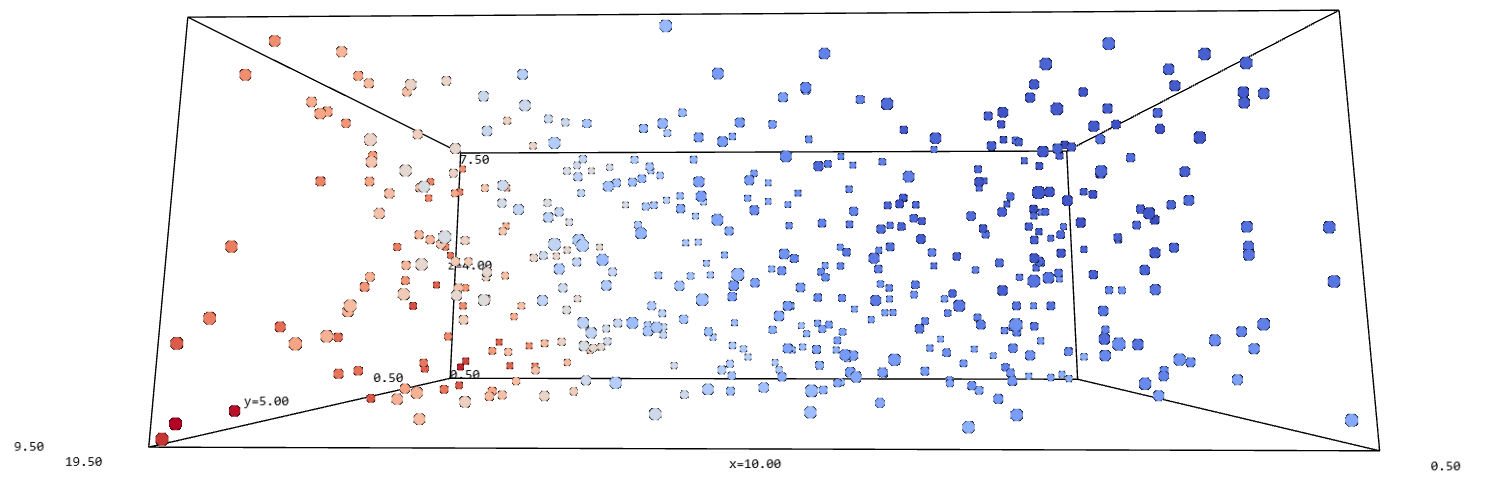
\includegraphics[width=\linewidth]{images/implicit.png}
    \caption{Implicit plot of all 500 color coded points. Red indicates high values, blue indicates low values.}
\end{figure}




\end{document}